\subsection{Thanh toán}
\subsubsection{Use case UML}
 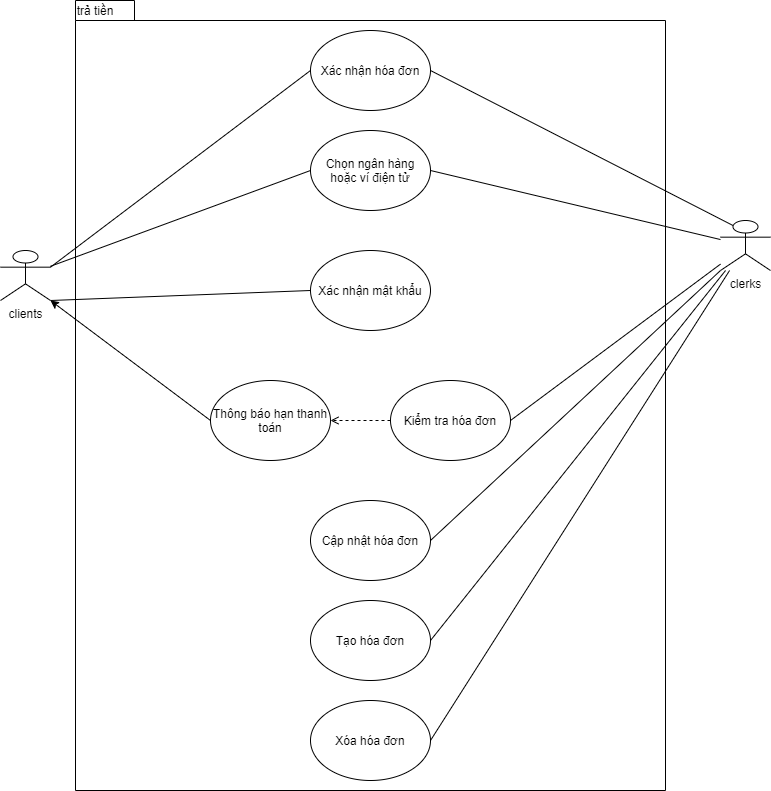
\includegraphics[scale=0.6]{Images/SE_UML-payment.png}

\subsubsection{Dặc tả}
\begin{center}{\color{black}}

    \begin{tabular}{|p{5cm}|p{7cm}|} \hline
    
        \textbf{Use Case Id} & \textbf{}  \\ \hline
        Tên usecase &  Trả tiền\\ \hline
        Tiền điều kiện & Người dùng xác nhận đặt món.\\ \hline
        
        
        Hậu điều kiện &  Người dùng thanh toán khoản nợ.\\ \hline
        Luồng điều kiện chính &  
            \begin{enumerate}
                \item App tạo khoản nợ.
                \item Người dùng yêu cầu thanh toán hóa đơn hoặc quá hạn thanh toán.
                \item App yêu cầu chọn ngân hàng, ví điện tử.
                \item App yêu cầu nhập số tài khoản hoặc quét mã QR.
                \item App yêu cầu xác nhận số tiền.
				\item Xác nhận mật khẩu.
				\item Xác nhận giao dịch.
				\item Xảy ra lỗi, yêu cầu khác hàng thực hiện lại từ bước 4
				\item Thông báo thành công, xóa khoản nợ của khách hàng.
            \end{enumerate}\\
        \hline
        Ngoại lệ & Người dùng hủy thực đơn \\ \hline
        Luồng điều kiện phụ & \\ \hline
      
    \end{tabular}
\end{center}
